% This file was created by tikzplotlib v0.8.5.
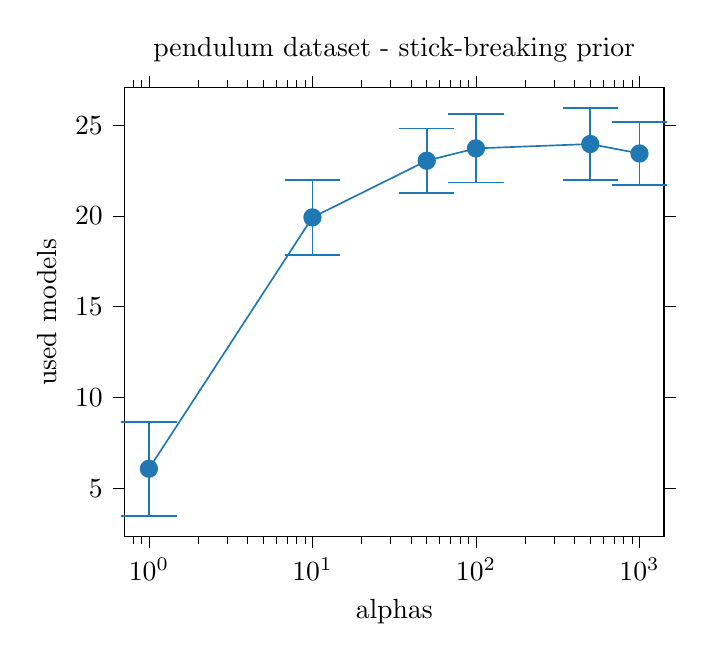
\begin{tikzpicture}

\definecolor{color0}{rgb}{0.12156862745098,0.466666666666667,0.705882352941177}

\begin{axis}[
log basis x={10},
tick align=outside,
tick pos=both,
title={pendulum dataset - stick-breaking prior },
x grid style={white!69.01960784313725!black},
xlabel={alphas},
xmin=0.707945784384138, xmax=1412.53754462275,
xmode=log,
xtick style={color=black},
y grid style={white!69.01960784313725!black},
ylabel={used models},
ymin=2.36691709456139, ymax=27.0513867269409,
ytick style={color=black}
]
\path [draw=color0, semithick]
(axis cs:1,3.48893844148774)
--(axis cs:1,8.67106155851226);

\path [draw=color0, semithick]
(axis cs:10,17.8430792022805)
--(axis cs:10,21.9969207977195);

\path [draw=color0, semithick]
(axis cs:50,21.2628112086782)
--(axis cs:50,24.8171887913218);

\path [draw=color0, semithick]
(axis cs:100,21.8327798220663)
--(axis cs:100,25.6072201779337);

\path [draw=color0, semithick]
(axis cs:500,21.9906346199854)
--(axis cs:500,25.9293653800146);

\path [draw=color0, semithick]
(axis cs:1000,21.7176759886711)
--(axis cs:1000,25.1623240113289);

\addplot [semithick, color0, mark=-, mark size=10, mark options={solid}, only marks]
table {%
1 3.48893844148774
10 17.8430792022805
50 21.2628112086782
100 21.8327798220663
500 21.9906346199854
1000 21.7176759886711
};
\addplot [semithick, color0, mark=-, mark size=10, mark options={solid}, only marks]
table {%
1 8.67106155851226
10 21.9969207977195
50 24.8171887913218
100 25.6072201779337
500 25.9293653800146
1000 25.1623240113289
};
\addplot [semithick, color0, mark=*, mark size=3, mark options={solid}]
table {%
1 6.08
10 19.92
50 23.04
100 23.72
500 23.96
1000 23.44
};
\end{axis}

\end{tikzpicture}
